\chapter{Technology studies}

The technology studies covers the studies leading up to the design and implementation. The technology studies help give an overview of how to realise the power line communication bus by providing good knowledge into the theory needed. During the technology studies the procedure were:
\begin{enumerate}
\item Discover literature
\item Create overview
\item Read and understand
\item Experiment
\end{enumerate}


\section{Protocol and communications}


\section{Clock and data recovery}
Normally a data transmission consists of two elements, clock and data. In this system that is not possible and therefore the area of clock and data recovery was investigated.

\subsection{What is clock recovery?}
Clock recovery is achieved essentially by extracting the clock from the incoming data stream. Due to the level shifts of the bitstream the clock is carried in the data.
\fixme{Skrives noget mere til hvad clock recovery er}

\subsection{The Phase-locked loop}
The phase-locked loop(PLL) comes in a large variety of designs but they all have one common conceptual diagram. A PLL consists of a phase-detector, a filter and a voltage controlled oscillator(VCO). Optionally it can contain a clock divider as well to speed up the VCO clock. Below on figure \ref{fig:conceptualpll} is shown the structure of the conceptual PLL.

\begin{figure}[H]
	\centering
	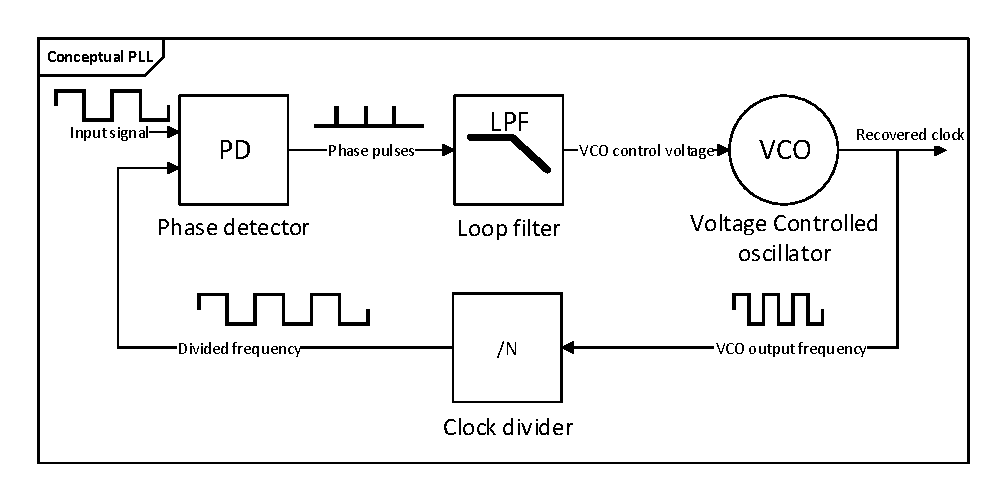
\includegraphics[width=.9\textwidth]{billeder/10technologystudies/conceptualpll}
	\caption{Conceptual PLL}
	\label{fig:conceptualpll}
\end{figure}

\subsubsection{Phase detector and loop filter}
The phase detector has two inputs. The input signal and the loop feedback signal. The phase detector compares the two input and produces a series of phase pulses depending on the phase difference of the two input signals. There is a vareity of different phase detector but two types are so common they are named type 1 and type 2 phase detectors. Each type of detector has an impact on how the loop locks and at what phase.
\\ \textbf{Type 1:}\\
The type 1 phase detector is basically a XOR gate. 

\begin{figure}[H]
	\centering
	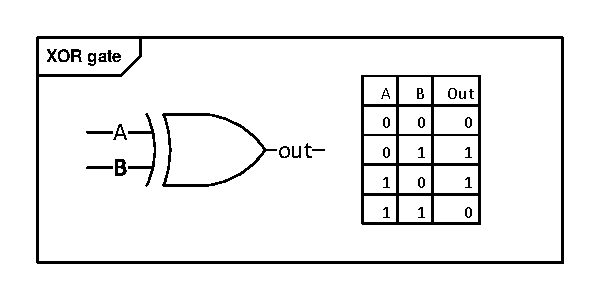
\includegraphics[width=.6\textwidth]{billeder/10technologystudies/XORgate}
	\caption{XOR gate}
	\label{fig:XOR}
\end{figure}

The XOR gate outputs a digital high when the two input signals are different from one another and a digital low when the two input signals are in the same state. Below on figure \ref{fig:pd1_waveforms} is shown the waveforms produced by a type 1 phase detector.
\begin{figure}[H]
	\centering
	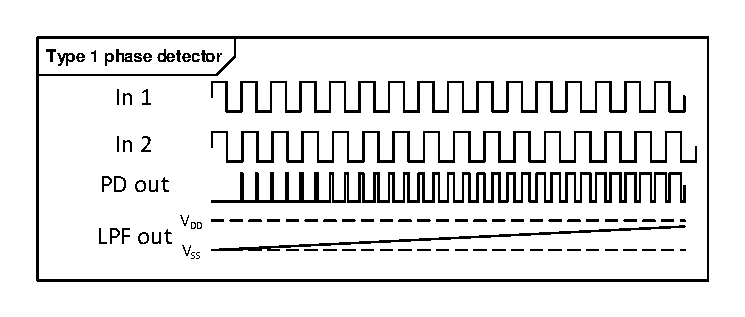
\includegraphics[width=.8\textwidth]{billeder/10technologystudies/PD1_waveforms}
	\caption{Phase detector type 1 waveforms}
	\label{fig:pd1_waveforms}
\end{figure}

The two input signals are out of frequency. And on the PD out line it is shown how this changes with regards to the two inputs.  The output of the low pass filter i used as an input to the VCO to either speed up the clock or slow it down.\\
When the PLL is in lock the LPF output will be $\frac{\text{V}_{\text{DD}}}{2}$. This effectively means that when the PLL locks on the In 1 signal the In 2 signal will be in exactly 90$^{\circ}$ deg phase.\\
\textbf{Type 2:}\\
The type 2 phase detector comprises of a phase comparator and a charge pump. The comparator is basically two D type flip-flops connected with and AND gate as seen on the figure \ref{fig:pd2_imp} below. The output from the phase comparator controls the charge pump to either charge or discharge the filter.

\begin{figure}[H]
	\centering
	\includegraphics[width=.7\textwidth]{billeder/10technologystudies/pd2_imp}
	\caption{Phase detector type 2 functional figure}
	\label{fig:pd2_imp}
\end{figure}

The advantage for the type 2 phase detector is the ability to detect a lead or a lag in frequency. Below on figure \ref{fig:pd2_waveform}, the waveform is illustrated for both leading and lagging. Depending on the amount of lead og lag the pump will be on/off for longer or lower periods of time.

\begin{figure}[H]
	\centering
	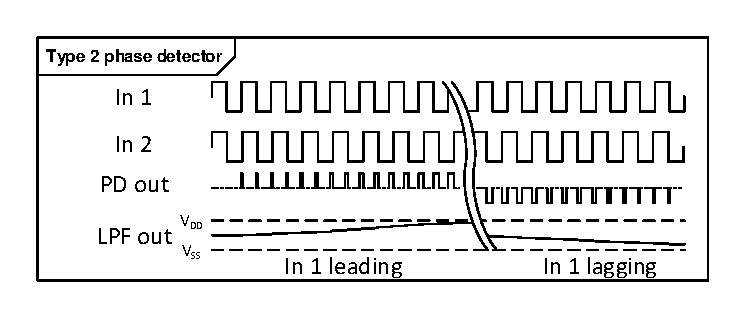
\includegraphics[width=.8\textwidth]{billeder/10technologystudies/pd2_waveform}
	\caption{Phase detector type 2 waveforms}
	\label{fig:pd2_waveform}
\end{figure}

\subsubsection{Voltage controlled oscillator and Clock divider}
The voltage controlled oscillator serves to convert the voltage output of the low pass filter to an output frequency. Below on figure \ref{fig:VCO_func} is shown the conceptual relationship between voltage input and frequency output.

\begin{figure}[H]
	\centering
	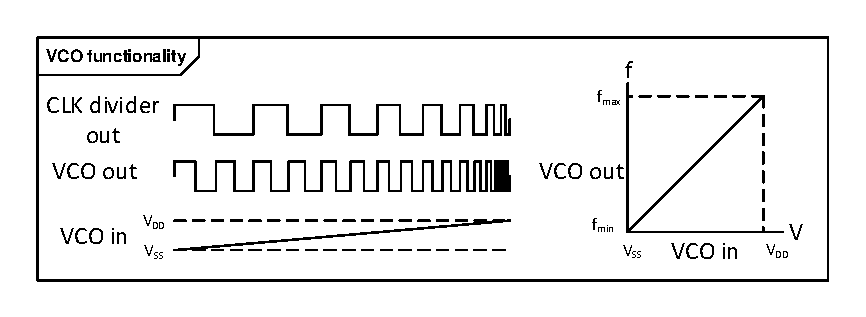
\includegraphics[width=1\textwidth]{billeder/10technologystudies/VCO_functionality}
	\caption{Voltage controlled oscillator functionality}
	\label{fig:VCO_func}
\end{figure}



